\chapter{引言}\label{chap:introduction}
粒子物理是关于基本粒子理论的学科,基本粒子的定义是不再可分的粒子。
粒子可不可分取决于“探针”的空间分辨率($\Delta r$),假设“探针”由点粒子组成,那么分辨率由德布罗意波长($\lambda=h/p$)决定。
在一台光学显微镜中,其分辨率为:
\begin{equation}
 \Delta r\approx \lambda/sin\theta
\end{equation}
代入德布罗意公式,得到:
\begin{equation}
 \Delta r\approx \frac{h}{psin\theta}\approx \frac{h}{q}
\end{equation}
可以发现,$\Delta r$与转移给光子或者其他入射粒子的动量($q$)成反比,那么对于$qc=10$ GeV的动量转移,
相应的空间分辨率大约为$10^{-16}$ m, 大约只有质子半径的十分之一。
所以想要看的越小,就需要更高的能量\footnote{在本文将采用的自然单位制中,可以更直接的看到这一联系:1 $\text{GeV}^{-1}\approx 0.2$ fm。}。
粒子物理就是伴随着加速器发展起来的,在20世纪早期,质子、中子曾作为基本粒子,因为当时的加速器能量只能达到几MeV,
随着加速器能量的提高,更多的粒子被发现,盖尔曼等人提出夸克模型以解释新发现的粒子\cite{GELLMANN1964214,Zweig:352337,Zweig:570209},并从70年代开始,所谓的标准模型(SM)在格拉肖等人的努力下建立起来\cite{GLASHOW1961579,PhysRevLett.19.1264,PhysRev.136.B763,PhysRevLett.30.1343,THOOFT1972189}。

标准模型是描述基本粒子和相互作用的理论(未包括引力作用),它成功预言或解释了大多数目前观测到的实验现象。
根据标准模型,物质世界由自旋为1/2的费米子组成,包括夸克($u, d, c, s, t, b$)和轻子($e, \mu, \tau, \nu_e, \nu_{\mu}, \nu_{\tau}$)。
%相互作用分为强(通过胶子传递),电磁(通过光子传递)和弱相互作用(通过$W/Z$传递)。
标准模型基本粒子总结在图\ref{fig:SM_particles}。
\begin{figure}
 \centering
 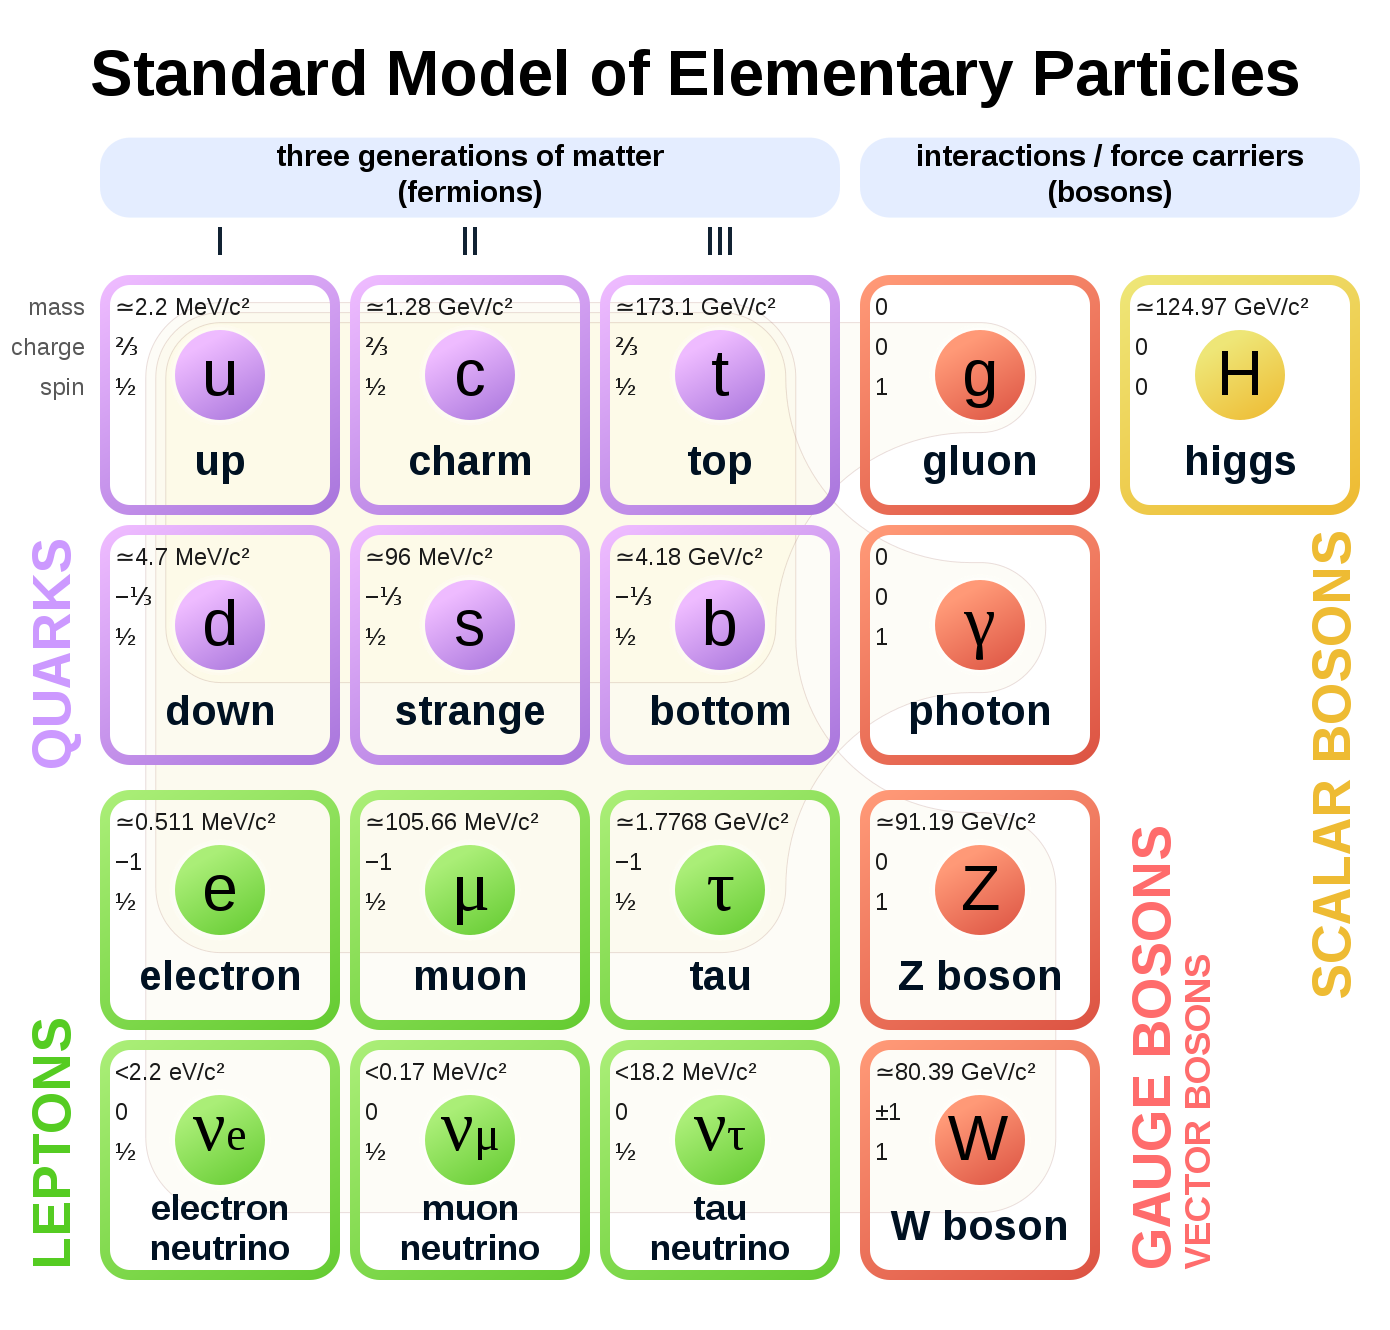
\includegraphics[width=0.75\textwidth]{fig/SM_particles.png}
 \caption{标准模型基本粒子总结。}
 \label{fig:SM_particles}
\end{figure}

标准模型是基于$SU(3)_C\bigotimes SU(2)_L\bigotimes U(1)_Y$群的规范场论,总共包含12个生成元。
每个生成元对应传递相互作用的一个规范玻色子,其中八个是胶子,为对称群为$SU(3)_C$的强相互作用传播子;
另外四个是$\gamma, W^{\pm}, Z$,为对称群为$SU(2)_L\bigotimes U(1)_Y$的电弱相互作用传播子。
为了保持规范对称性,这些中间传播子应当是无质量的。
夸克间的强相互作用由量子色动力学(QCD)描述,它具有渐近自由和夸克禁闭的性质。
电磁和弱作用由电弱统一理论(EW)描述,其中电磁相互作用通过光子传递,弱作用通过$W^{\pm}, Z$传递。
每种相互作用有不同的力程和强度,总结如表\ref{tab:summary_interactions}所示\footnote{弱相互作用常数具有GeV$^{-2}$量纲,为方便比较,乘上质子质量平方,引力作用常数也使用质子质量。} 。
弱作用的短力程和长作用时间表明中间玻色子($W^{\pm}, Z$)是有质量的,而这与规范对称性矛盾。
\begin{table}[h]
\centering
\begin{tabular}{c|c|c|c|c}
\hline
     		&强相互作用   &电磁相互作用  &弱相互作用 &引力相互作用 \\
\hline
源		&色荷  &电荷   &弱超荷   &质量 \\
相互作用常数 &$1\sim 10$  &$\approx$1/137   &$\approx 1\times 10^{-5}$    &$5\times 10^{-40}$ \\
力的传递者 &胶子  &光子  &$W^{\pm}, Z$  &- \\
典型作用时间(s) &$10^{-23}$  &$10^{-16}$  &$10^{-10}$   &- \\
力程  &1 fm  &$\infty$   &1/400 fm  &$\infty$  \\
\hline
\end{tabular}
\caption{四种相互作用特征表。}
\label{tab:summary_interactions}
\end{table}

希格斯机制\cite{PhysRevLett.13.321,HIGGS1964132,PhysRevLett.13.508,PhysRevLett.13.585,PhysRev.145.1156,PhysRev.155.1554}保持了理论的规范对称性,同时通过自发对称性破缺使得中间玻色子获得了质量,并且预言了一个新的标量粒子,即希格斯粒子。
经过几十年的寻找,希格斯粒子于2012年在LHC发现\cite{Aad:2012tfa,Chatrchyan:2012xdj}。虽然截止目前对希格斯粒子的测量并未发现明显超出标准模型迹象,但是误差较大。
精确测量希格斯粒子性质是非常重要的,因为任何的偏差会给新物理寻提供线索。顶夸克的汤川耦合是希格斯粒子测量的重要目标,顶夸克在标准模型中具有最大的质量,
理论表明它与希格斯粒子的汤川耦合是最强的,所以实验与理论的偏差有可能是新物理的迹象。
希格斯粒子关联顶夸克对产生模式($t\bar{t}h$)是这一测量的黄金过程,虽然$t\bar{t}h$产生截面只占希格斯粒子总产生截面的1\%,但是\RunTwo 是\RunOne 的几乎四倍,
为寻找$t\bar{t}h$提供了可能。

与夸克和轻子不同,希格斯粒子具有一独特的性质,即自耦合,自耦合常数的测量可以帮助验证和更深一步理解希格斯机制。
通过测量希格斯粒子对的产生可以帮助限制自耦合常数范围。
而且在许多新物理模型中,通过修改自耦合常数或者增加一个希格斯二重态可以增大希格斯粒子对的产生截面,
所以对希格斯粒子对的寻找也能帮助寻找新物理。

标准模型希格斯粒子多种衰变渠道,主要到$b\bar{b}$, $ZZ$, $\tau\tau$等。$h\rightarrow b\bar{b}$虽然有最高的分支比(58\%),但是在强子对撞机容易淹没在海量的喷注本底中。
而$h\rightarrow WW/\tau\tau$可为希格斯粒子提供标记,得益于它们的轻子末态或者强子化衰变的$\tau_{\text{had}}$。本文将论述通过多轻子道寻找$t\bar{t}h$和希格斯粒子对,结构如下:
第\ref{chap:higgs_pheno}章简要介绍希格斯唯象学,包括LHC单希格斯粒子产生,双希格斯粒子产生以及类希格斯对产生;
第\ref{chap:lhc_atlas}章首先描述LHC和ATLAS探测器,随后介绍ATLAS实验事例重建,事例仿真等过程,最后介绍ATLAS Phase-II升级以及
硅微条探测器模块组装和测试;
第\ref{chap:tth_multilep}章论述通过多轻子道寻找$t\bar{t}h$产生,主要关注由单轻子和两$\tau_{\text{had}}$的组成的信号道的数据分析过程,并给出统计结果;
第\ref{chap:hh_serach}章展示通过多轻子道寻找希格斯粒子对和类希格斯对产生,重点论述相同电荷双轻子分析道,最后给出统计结果;
第\ref{chap:conclusions}章作出文章总结,并对未来的分析工作作出一定展望。
